\documentclass[11pt]{article}
\usepackage[a4paper,margin=1in]{geometry}
\usepackage{amsmath,amssymb,amsthm}
\usepackage{tikz}
\usetikzlibrary{arrows.meta,calc}
\usepackage{xcolor}
\usepackage[hidelinks]{hyperref}
\hypersetup{pdftitle={Even and odd Dyck paths},pdfauthor={Vamshi Jandhyala}}
\setlength{\parskip}{0.4em}
\setlength{\parindent}{0pt}

\newtheorem{theorem}{Theorem}
\newtheorem{lemma}{Lemma}
\theoremstyle{remark}
\newtheorem*{remark}{Remark}

\definecolor{inkblue}{RGB}{40,76,105}
\definecolor{softblue}{RGB}{226,235,243}
\definecolor{rust}{RGB}{153,70,45}

\newcommand{\maj}{\operatorname{maj}}
\newcommand{\w}[1]{\texttt{#1}}

\title{Even and odd Dyck paths}
\author{Vamshi Jandhyala}
\date{}

\begin{document}
\maketitle
\vspace{-2em}

\begin{abstract}
Weight a Dyck path by the sum of the positions of its valleys. Among the paths of semilength
$n$ with $k$ valleys, those of even weight outnumber those of odd weight, and Johann Cigler
observed that the excess is exactly the number of symmetric paths with $k$ valleys. He proved
it by evaluating $q$-Narayana numbers at $q=-1$ and asked for a combinatorial proof. This note
gives one. Valley coordinates turn each path into a Motzkin word in which the sign is a product
of local signs; swapping letters inside pairs cancels every word except some of sign $+1$; and
a halving map matches those survivors with the symmetric paths. The survivors are not the
symmetric paths themselves, and cannot be: for odd $n$ and $k$ every symmetric path is odd. The
argument has been checked in the Lean proof assistant.
\end{abstract}

\section{Five paths}

A \emph{Dyck path} of semilength $n$ is a sequence of $n$ up steps $U$ and $n$ down steps
$D$ that never goes below its starting level. A \emph{valley} is a down step followed at once
by an up step; its \emph{position} is the number of that down step, counting from $1$. The
\emph{major index} $\maj P$ is the sum of the positions of the valleys of $P$. Figure~\ref{fig:three}
shows the five paths of semilength $3$.

\begin{figure}[ht]
\centering
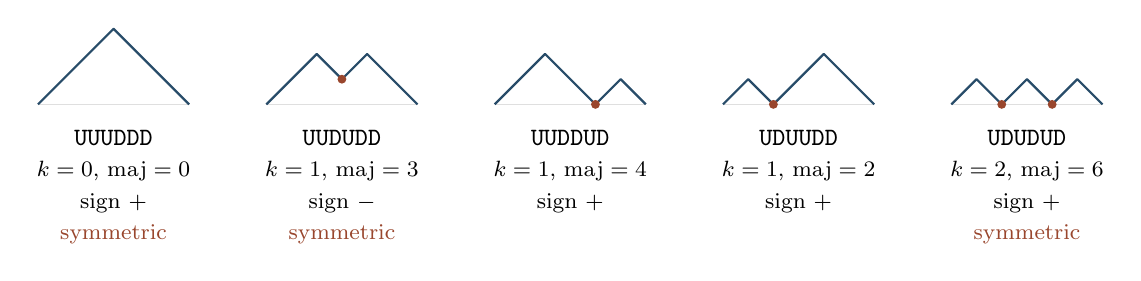
\begin{tikzpicture}[line join=round]
\draw[gray!25] (0.0,0) -- (1.92,0);
\draw[thick,inkblue] (0.000,0.000) -- (0.320,0.320) -- (0.640,0.640) -- (0.960,0.960) -- (1.280,0.640) -- (1.600,0.320) -- (1.920,-0.000);
\node[font=\small] at (0.96,-0.42) {\texttt{UUUDDD}};
\node[font=\footnotesize] at (0.96,-0.85) {$k=0$, $\maj=0$};
\node[font=\footnotesize] at (0.96,-1.25) {sign $+$};
\node[font=\footnotesize,rust] at (0.96,-1.65) {symmetric};
\draw[gray!25] (2.9,0) -- (4.82,0);
\draw[thick,inkblue] (2.900,0.000) -- (3.220,0.320) -- (3.540,0.640) -- (3.860,0.320) -- (4.180,0.640) -- (4.500,0.320) -- (4.820,0.000);
\fill[rust] (3.860,0.320) circle (1.6pt);
\node[font=\small] at (3.86,-0.42) {\texttt{UUDUDD}};
\node[font=\footnotesize] at (3.86,-0.85) {$k=1$, $\maj=3$};
\node[font=\footnotesize] at (3.86,-1.25) {sign $-$};
\node[font=\footnotesize,rust] at (3.86,-1.65) {symmetric};
\draw[gray!25] (5.8,0) -- (7.72,0);
\draw[thick,inkblue] (5.800,0.000) -- (6.120,0.320) -- (6.440,0.640) -- (6.760,0.320) -- (7.080,0.000) -- (7.400,0.320) -- (7.720,0.000);
\fill[rust] (7.080,0.000) circle (1.6pt);
\node[font=\small] at (6.76,-0.42) {\texttt{UUDDUD}};
\node[font=\footnotesize] at (6.76,-0.85) {$k=1$, $\maj=4$};
\node[font=\footnotesize] at (6.76,-1.25) {sign $+$};
\draw[gray!25] (8.7,0) -- (10.62,0);
\draw[thick,inkblue] (8.700,0.000) -- (9.020,0.320) -- (9.340,0.000) -- (9.660,0.320) -- (9.980,0.640) -- (10.300,0.320) -- (10.620,0.000);
\fill[rust] (9.340,0.000) circle (1.6pt);
\node[font=\small] at (9.66,-0.42) {\texttt{UDUUDD}};
\node[font=\footnotesize] at (9.66,-0.85) {$k=1$, $\maj=2$};
\node[font=\footnotesize] at (9.66,-1.25) {sign $+$};
\draw[gray!25] (11.6,0) -- (13.52,0);
\draw[thick,inkblue] (11.600,0.000) -- (11.920,0.320) -- (12.240,0.000) -- (12.560,0.320) -- (12.880,0.000) -- (13.200,0.320) -- (13.520,0.000);
\fill[rust] (12.240,0.000) circle (1.6pt);
\fill[rust] (12.880,0.000) circle (1.6pt);
\node[font=\small] at (12.559999999999999,-0.42) {\texttt{UDUDUD}};
\node[font=\footnotesize] at (12.559999999999999,-0.85) {$k=2$, $\maj=6$};
\node[font=\footnotesize] at (12.559999999999999,-1.25) {sign $+$};
\node[font=\footnotesize,rust] at (12.559999999999999,-1.65) {symmetric};
\end{tikzpicture}

\caption{The Dyck paths of semilength $3$. Valleys are marked; $k$ is the number of valleys and
the sign is $(-1)^{\maj}$. A path is symmetric when it equals its mirror image, read backwards
with $U$ and $D$ exchanged.}
\label{fig:three}
\end{figure}

Stop and try this before reading on. Sort the paths of Figure~\ref{fig:three} by their number
of valleys. In each group, subtract the number of paths with odd major index from the number
with even major index. Then count the symmetric paths in each group.

Both counts give $1, 1, 1$. In the middle group the major indices are $3$, $4$ and $2$, so the
signed count is $1+1-1=1$, and there is one symmetric path. Write $E_{n,k}$ and $O_{n,k}$ for
the numbers of paths of semilength $n$ with $k$ valleys and even or odd major index, and
$S_{n,k}$ for the number of symmetric ones.

\begin{theorem}\label{thm:main}
For all $n\ge 1$ and $k\ge 0$, \ $E_{n,k}-O_{n,k}=S_{n,k}$.
\end{theorem}

Why should anyone care? The number of Dyck paths with $k$ valleys is a Narayana number, and
F\"urlinger and Hofbauer~\cite{FH} found its natural $q$-analogue:
\begin{equation}\label{eq:FH}
\sum_{P}q^{\maj P}\;=\;q^{k(k+1)}\,\frac{1}{[k+1]_q}\binom{n}{k}_{\!q}\binom{n-1}{k}_{\!q},
\end{equation}
the sum running over the paths of semilength $n$ with $k$ valleys. The left side lists the
paths by major index. The right side is the familiar product formula for the Narayana number,
$\frac{1}{k+1}\binom{n}{k}\binom{n-1}{k}$, with each integer replaced by its $q$-analogue
$[m]_q=1+q+\dots+q^{m-1}$, and a power of $q$ in front. Putting $q=-1$ on the left gives
$E_{n,k}-O_{n,k}$, since $k(k+1)$ is even. Cigler~\cite{Cig26} evaluated the right side at $q=-1$
and counted symmetric paths, finding they agree; on MathOverflow~\cite{MO} he asked for a direct
combinatorial proof, and Peter Taylor pointed out there that it amounts to Theorem~\ref{thm:main}.
Identities of this shape, a $q$-count at $q=-1$ equal to the number of objects fixed by an
involution, are instances of Stembridge's $q=-1$ phenomenon~\cite{Stem}. For even $n$ the same
value is also the half-turn case of a cyclic sieving theorem of Reiner, Stanton and
White~\cite[Theorem 7.2]{RSW}, which counts noncrossing partitions; that proof, too, computes both
sides. What follows is a direct argument for every $n$.

\section{A tempting pairing that fails}

The first idea is to pair each path with its mirror image $P^*$. It does not work, and seeing
why shapes everything later.

A valley of $P$ at position $p$ consists of a down step at $p$ and an up step at $p+1$. Reading
backwards and exchanging the letters turns these into an up step at $2n+1-p$ and a down step at
$2n-p$: a valley of $P^*$ at position $2n-p$. So
\[
\maj P^*=2nk-\maj P,
\]
which has the same parity as $\maj P$. Mirror pairs never cancel. Worse, the valleys of a
symmetric path come in pairs $p$ and $2n-p$ (with $p=n$ unpaired), so a symmetric path has
$\maj P=nk$. When $n$ and $k$ are both odd, every symmetric path has odd major index and counts
$-1$ on the left of Theorem~\ref{thm:main}, while it is meant to count $+1$ on the right. The path
\w{UUDUDD} of Figure~\ref{fig:three} is the smallest example.

So a cancellation argument has to throw away some symmetric paths and keep some that are not
symmetric, and then match the survivors with the symmetric paths by a separate bijection. In
Figure~\ref{fig:three} the argument below cancels \w{UUDUDD} against \w{UDUUDD} and keeps
\w{UUDDUD}.

\section{Valleys as coordinates}

The sign $(-1)^{\maj P}$ depends on the positions of all the valleys at once. The first step is a
change of description that makes it a product of local pieces.

Look at the path on the left of Figure~\ref{fig:encode}. Its valleys are at positions $3$ and $8$.
The valley at $3$ has $2$ up steps before it and is the $1$st down step; the valley at $8$ has $4$
up steps before it and is the $4$th down step. The positions are the sums: $3=2+1$ and $8=4+4$.

\begin{figure}[ht]
\centering
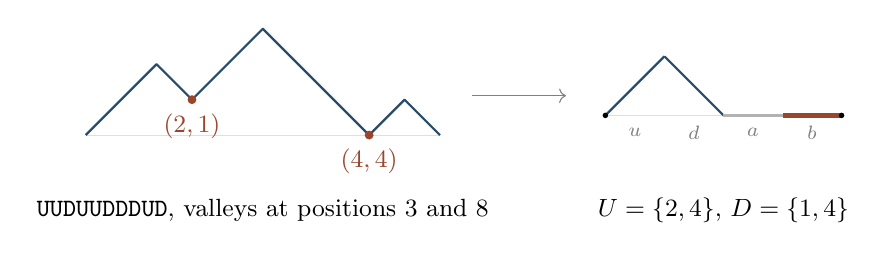
\begin{tikzpicture}[line join=round]
\draw[gray!25] (0,0) -- (4.5,0);
\draw[thick,inkblue] (0.000,0.000) -- (0.450,0.450) -- (0.900,0.900) -- (1.350,0.450) -- (1.800,0.900) -- (2.250,1.350) -- (2.700,0.900) -- (3.150,0.450) -- (3.600,0.000) -- (4.050,0.450) -- (4.500,0.000);
\fill[rust] (1.350,0.450) circle (1.6pt);
\fill[rust] (3.600,0.000) circle (1.6pt);
\node[font=\small,rust,below] at (1.350,0.400) {$(2,1)$};
\node[font=\small,rust,below] at (3.600,-0.050) {$(4,4)$};
\node[font=\small] at (2.25,-0.95) {\texttt{UUDUUDDDUD}, valleys at positions 3 and 8};
\draw[->,gray] (4.9,0.5) -- (6.1,0.5);
\draw[gray!25] (6.6,0.25) -- (9.6,0.25);
\draw[thick,inkblue] (6.600,0.250) -- (7.350,1.000);
\node[font=\scriptsize,gray] at (6.975,0.030) {$u$};
\draw[thick,inkblue] (7.350,1.000) -- (8.100,0.250);
\node[font=\scriptsize,gray] at (7.725,0.030) {$d$};
\draw[thick,gray!60] (8.100,0.250) -- (8.850,0.250);
\node[font=\scriptsize,gray] at (8.475,0.030) {$a$};
\draw[ultra thick,rust] (8.850,0.250) -- (9.600,0.250);
\node[font=\scriptsize,gray] at (9.225,0.030) {$b$};
\fill (6.600,0.250) circle (1pt);
\fill (9.600,0.250) circle (1pt);
\node[font=\small] at (8.1,-0.95) {$U=\{2,4\}$, $D=\{1,4\}$};
\end{tikzpicture}

\caption{A path, its valley coordinates $(u_j,d_j)$, and its word. Reading $x=1,2,3,4$: $x$ is in
$D$ only, in $U$ only, in neither, in both, giving the letters $u$, $d$, $a$, $b$. The word is
drawn as a path: $u$ and $d$ go up and down, $a$ is a grey level step, $b$ a thick rust one.}
\label{fig:encode}
\end{figure}

In general, for the $j$th valley let $u_j$ be the number of up steps before it and $d_j$ the
number of down steps up to and including it. Its position is $u_j+d_j$, so
\begin{equation}\label{eq:maj}
\maj P=\sum_{j=1}^k u_j+\sum_{j=1}^k d_j .
\end{equation}
In words, the major index splits into a contribution from the up steps and one from the down
steps. The height of the path at the $j$th valley is $u_j-d_j$.

\begin{lemma}\label{lem:coords}
Let $n\ge1$. The valley coordinates of a Dyck path of semilength $n$ with $k$ valleys satisfy
\[
1\le u_1<\dots<u_k\le n-1,\qquad 1\le d_1<\dots<d_k\le n-1,\qquad d_j\le u_j\ \text{for all } j,
\]
and every such pair of sequences comes from exactly one Dyck path.
\end{lemma}

\begin{proof}
Between consecutive valleys a path makes one run of up steps and then one run of down steps,
so $P=U^{u_1}D^{d_1}U^{u_2-u_1}D^{d_2-d_1}\cdots U^{n-u_k}D^{n-d_k}$. Every run is nonempty,
which says that the sequences increase strictly and that $u_k$ and $d_k$ are less than $n$
(after the last valley there are still up steps and down steps to come). Conversely this formula
builds a sequence of $n$ steps of each kind from any two such sequences. Its lowest points are
its valleys and its end, so it stays at or above its starting level exactly when every valley
height $u_j-d_j$ is at least $0$.
\end{proof}

Put $U=\{u_1,\dots,u_k\}$ and $D=\{d_1,\dots,d_k\}$, both subsets of $\{1,\dots,n-1\}$, and write
a word $w$ of length $n-1$ whose $x$th letter records whether $x$ lies in $D$ or $U$:
\[
w_x=u \text{ if } x\in D\setminus U,\qquad d \text{ if } x\in U\setminus D,\qquad a \text{ if } x\notin U\cup D,
\qquad b \text{ if } x\in U\cap D .
\]
Read $u$ and $d$ as up and down steps and $a$, $b$ as two kinds of level step, as in
Figure~\ref{fig:encode}. The names are chosen so that the condition $d_j\le u_j$ becomes a familiar
one.

\begin{lemma}\label{lem:word}
The words of Dyck paths of semilength $n$ with $k$ valleys are exactly the words of length $n-1$
over $\{u,d,a,b\}$ that never go below their starting level, end at it, and have $k$ letters
from $\{u,b\}$. Moreover
\begin{equation}\label{eq:sign}
(-1)^{\maj P}=\prod_{x:\ w_x\in\{u,d\}}(-1)^x ,
\end{equation}
and $P$ is symmetric exactly when $w$ read backwards, with $u$ and $d$ exchanged, is $w$ again.
\end{lemma}

\begin{proof}
After $x$ letters the word has risen $|D\cap[1,x]|-|U\cap[1,x]|$, the number of $d_j$ up to $x$
minus the number of $u_j$ up to $x$. If $d_j\le u_j$ for all $j$, then each $u_j\le x$ brings a
$d_j\le x$ with it, so this is never negative. Conversely, taking $x=u_j$ gives at least $j$
values $d_i\le u_j$, so $d_j\le u_j$. The word ends at its starting level because $|U|=|D|=k$,
and the letters from $\{u,b\}$ are the elements of $D$, so there are $k$ of them.
Lemma~\ref{lem:coords} turns these word conditions back into a unique path.

For~\eqref{eq:sign}, each $x$ in exactly one of $U$ and $D$ appears once in~\eqref{eq:maj}, and
each $x$ in both appears twice, contributing $(-1)^{2x}=1$.

For the mirror image, the valley at position $p_j=u_j+d_j$ becomes the valley at $2n-p_j$, which
has $n-d_j$ up steps before it and is the $(n-u_j)$th down step. So $P^*$ has $U^*=n-D$ and $D^*=n-U$:
its $x$th letter is the $(n-x)$th letter of $w$ with $u$ and $d$ exchanged.
\end{proof}

Equation~\eqref{eq:sign} is the point of the change. Each up or down letter carries the sign of
its position and the level letters carry nothing. The five paths of Figure~\ref{fig:three} have
the words $aa$, $ud$, $ab$, $ba$ and $bb$, with signs $+$, $-$, $+$, $+$, $+$.

\section{Swapping inside pairs}

By~\eqref{eq:sign}, moving a single $u$ or $d$ by one place changes the sign. That suggests cutting
$w$ into pairs of letters at positions $2i-1$ and $2i$, leaving the last letter alone when $n-1$ is
odd, and looking for pairs that can be changed without disturbing anything else. Give some pairs a
\emph{partner} (Figure~\ref{fig:partners}):
\begin{itemize}
\item a pair with exactly one level letter, such as $ua$ or $bd$, is partnered with the same two
letters in the other order;
\item $ud$ is partnered with $ba$;
\item $du$ is partnered with $ab$, but only when the height before the pair is at least $1$.
\end{itemize}
The pairs $uu$, $dd$, $aa$, $bb$ have no partner, and neither has $ab$ at height $0$.

\begin{figure}[ht]
\centering
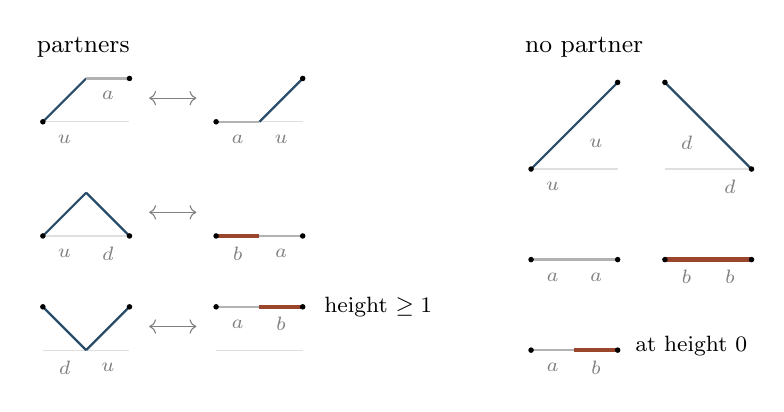
\begin{tikzpicture}[line join=round]
\node[font=\small,anchor=west] at (-0.2,0.95) {partners};
\draw[gray!25] (0,-0.0) -- (1.1,-0.0);
\draw[thick,inkblue] (0.000,0.000) -- (0.550,0.550);
\node[font=\scriptsize,gray] at (0.275,-0.220) {$u$};
\draw[thick,gray!60] (0.550,0.550) -- (1.100,0.550);
\node[font=\scriptsize,gray] at (0.825,0.330) {$a$};
\fill (0.000,0.000) circle (1pt);
\fill (1.100,0.550) circle (1pt);
\draw[<->,gray] (1.35,0.3) -- (1.95,0.3);
\draw[gray!25] (2.2,-0.0) -- (3.3000000000000003,-0.0);
\draw[thick,gray!60] (2.200,0.000) -- (2.750,0.000);
\node[font=\scriptsize,gray] at (2.475,-0.220) {$a$};
\draw[thick,inkblue] (2.750,0.000) -- (3.300,0.550);
\node[font=\scriptsize,gray] at (3.025,-0.220) {$u$};
\fill (2.200,0.000) circle (1pt);
\fill (3.300,0.550) circle (1pt);
\draw[gray!25] (0,-1.45) -- (1.1,-1.45);
\draw[thick,inkblue] (0.000,-1.450) -- (0.550,-0.900);
\node[font=\scriptsize,gray] at (0.275,-1.670) {$u$};
\draw[thick,inkblue] (0.550,-0.900) -- (1.100,-1.450);
\node[font=\scriptsize,gray] at (0.825,-1.670) {$d$};
\fill (0.000,-1.450) circle (1pt);
\fill (1.100,-1.450) circle (1pt);
\draw[<->,gray] (1.35,-1.15) -- (1.95,-1.15);
\draw[gray!25] (2.2,-1.45) -- (3.3000000000000003,-1.45);
\draw[ultra thick,rust] (2.200,-1.450) -- (2.750,-1.450);
\node[font=\scriptsize,gray] at (2.475,-1.670) {$b$};
\draw[thick,gray!60] (2.750,-1.450) -- (3.300,-1.450);
\node[font=\scriptsize,gray] at (3.025,-1.670) {$a$};
\fill (2.200,-1.450) circle (1pt);
\fill (3.300,-1.450) circle (1pt);
\draw[gray!25] (0,-2.9) -- (1.1,-2.9);
\draw[thick,inkblue] (0.000,-2.350) -- (0.550,-2.900);
\node[font=\scriptsize,gray] at (0.275,-3.120) {$d$};
\draw[thick,inkblue] (0.550,-2.900) -- (1.100,-2.350);
\node[font=\scriptsize,gray] at (0.825,-3.120) {$u$};
\fill (0.000,-2.350) circle (1pt);
\fill (1.100,-2.350) circle (1pt);
\draw[<->,gray] (1.35,-2.6) -- (1.95,-2.6);
\draw[gray!25] (2.2,-2.9) -- (3.3000000000000003,-2.9);
\draw[thick,gray!60] (2.200,-2.350) -- (2.750,-2.350);
\node[font=\scriptsize,gray] at (2.475,-2.570) {$a$};
\draw[ultra thick,rust] (2.750,-2.350) -- (3.300,-2.350);
\node[font=\scriptsize,gray] at (3.025,-2.570) {$b$};
\fill (2.200,-2.350) circle (1pt);
\fill (3.300,-2.350) circle (1pt);
\node[font=\footnotesize,anchor=west] at (3.45,-2.3499999999999996) {height $\ge 1$};
\node[font=\small,anchor=west] at (6.0,0.95) {no partner};
\draw[gray!25] (6.2,-0.6) -- (7.300000000000001,-0.6);
\draw[thick,inkblue] (6.200,-0.600) -- (6.750,-0.050);
\node[font=\scriptsize,gray] at (6.475,-0.820) {$u$};
\draw[thick,inkblue] (6.750,-0.050) -- (7.300,0.500);
\node[font=\scriptsize,gray] at (7.025,-0.270) {$u$};
\fill (6.200,-0.600) circle (1pt);
\fill (7.300,0.500) circle (1pt);
\draw[gray!25] (7.9,-0.6) -- (9.0,-0.6);
\draw[thick,inkblue] (7.900,0.500) -- (8.450,-0.050);
\node[font=\scriptsize,gray] at (8.175,-0.270) {$d$};
\draw[thick,inkblue] (8.450,-0.050) -- (9.000,-0.600);
\node[font=\scriptsize,gray] at (8.725,-0.820) {$d$};
\fill (7.900,0.500) circle (1pt);
\fill (9.000,-0.600) circle (1pt);
\draw[gray!25] (6.2,-1.75) -- (7.300000000000001,-1.75);
\draw[thick,gray!60] (6.200,-1.750) -- (6.750,-1.750);
\node[font=\scriptsize,gray] at (6.475,-1.970) {$a$};
\draw[thick,gray!60] (6.750,-1.750) -- (7.300,-1.750);
\node[font=\scriptsize,gray] at (7.025,-1.970) {$a$};
\fill (6.200,-1.750) circle (1pt);
\fill (7.300,-1.750) circle (1pt);
\draw[gray!25] (7.9,-1.75) -- (9.0,-1.75);
\draw[ultra thick,rust] (7.900,-1.750) -- (8.450,-1.750);
\node[font=\scriptsize,gray] at (8.175,-1.970) {$b$};
\draw[ultra thick,rust] (8.450,-1.750) -- (9.000,-1.750);
\node[font=\scriptsize,gray] at (8.725,-1.970) {$b$};
\fill (7.900,-1.750) circle (1pt);
\fill (9.000,-1.750) circle (1pt);
\draw[gray!25] (6.2,-2.9) -- (7.300000000000001,-2.9);
\draw[thick,gray!60] (6.200,-2.900) -- (6.750,-2.900);
\node[font=\scriptsize,gray] at (6.475,-3.120) {$a$};
\draw[ultra thick,rust] (6.750,-2.900) -- (7.300,-2.900);
\node[font=\scriptsize,gray] at (7.025,-3.120) {$b$};
\fill (6.200,-2.900) circle (1pt);
\fill (7.300,-2.900) circle (1pt);
\node[font=\footnotesize,anchor=west] at (7.4,-2.85) {at height $0$};
\end{tikzpicture}

\caption{Partners. A swap moves one up or down letter by one place; $ud$ and $ba$ both go
nowhere and both contain one letter from $\{u,b\}$; $du$ dips, so it needs height $1$ to stand on.}
\label{fig:partners}
\end{figure}

The rule is: find the first pair in $w$ that has a partner, and replace it by its partner. For
the word $udab$ of Figure~\ref{fig:encode} the first pair is $ud$, so the rule gives $baab$, the
word of \w{UDUUUDDDUD}. The major indices are $11$ and $10$.

\begin{lemma}\label{lem:swap}
The rule is an involution on the words of Lemma~\ref{lem:word} with $k$ letters from $\{u,b\}$.
When it moves a word, it changes its sign. A word it fixes has sign $+1$.
\end{lemma}

\begin{proof}
A pair and its partner rise by the same amount, so the heights before all later pairs are
unchanged; the earlier pairs have no partner and are untouched. Applying the rule again therefore
finds the same pair and puts it back. The new word is legal, because a swap changes only the height in
the middle of the pair. That middle height is the height before the pair when a level letter comes
first, the height after the pair when the level letter comes second, and one more than the height
before the pair for $ud$; all three are at least $0$ in a legal word. The remaining case is $du$,
whose middle height is one less than the height before it, and that is what the condition on its
partner allows for.
The number of letters from $\{u,b\}$ is kept, since $ud$ and $ba$ each have one, as do $du$ and $ab$.

For the sign, use~\eqref{eq:sign}. A swap moves one up or down letter between positions $2i-1$ and
$2i$, which flips its sign. The pairs $ud$ and $du$ contribute $(-1)^{2i-1}(-1)^{2i}=-1$, and the
pairs $ba$ and $ab$ contribute $+1$.

A fixed word consists of pairs $uu$, $dd$, $aa$, $bb$, and $ab$ at height $0$, followed perhaps by a
lone last letter. The lone letter is a level letter, because the pairs use an even number of up
and down letters and a word that returns to its start has as many $u$ as $d$, hence an even number
of them in all. Each $uu$ and each $dd$ contributes $-1$ to the sign, and there are as many of one
as of the other, because no other pair changes the height. So the sign is $+1$.
\end{proof}

Summing $(-1)^{\maj P}$ over all paths with $k$ valleys, the words moved by the rule cancel in
pairs, and so
\begin{equation}\label{eq:fixed}
E_{n,k}-O_{n,k}=\text{the number of fixed words with $k$ letters from $\{u,b\}$}.
\end{equation}
For $n=3$ the words are single pairs: $ud$ and $ba$ cancel, and the fixed words are $aa$, $ab$ and
$bb$, one in each group, as in Figure~\ref{fig:three}.

\section{From fixed words to symmetric paths}

The last step matches fixed words with mirror-symmetric words. Take the fixed word
$ab\,uu\,dd\,ab$ at the top of Figure~\ref{fig:halve}. Each of its pairs changes the height by $0$ or
$\pm2$, so the heights between pairs are even, and it can be halved: write one letter per pair, $uu\mapsto u$, $dd\mapsto d$, $aa\mapsto a$, $bb\mapsto b$, and
$ab\mapsto c$, a new level letter. The result $c\,u\,d\,c$ returns to its start and has $c$ only at
height $0$. Now turn each $c$ into $u$, giving $uudu$. This word never goes below its start, but it
no longer needs to end there. The steps that were $c$ have a description of their own: the first
is the last step leaving level $0$, the second the last step leaving level $1$. Finally append the
mirror image $dudd$, to get the symmetric word $uudu\,dudd$.

\begin{figure}[ht]
\centering
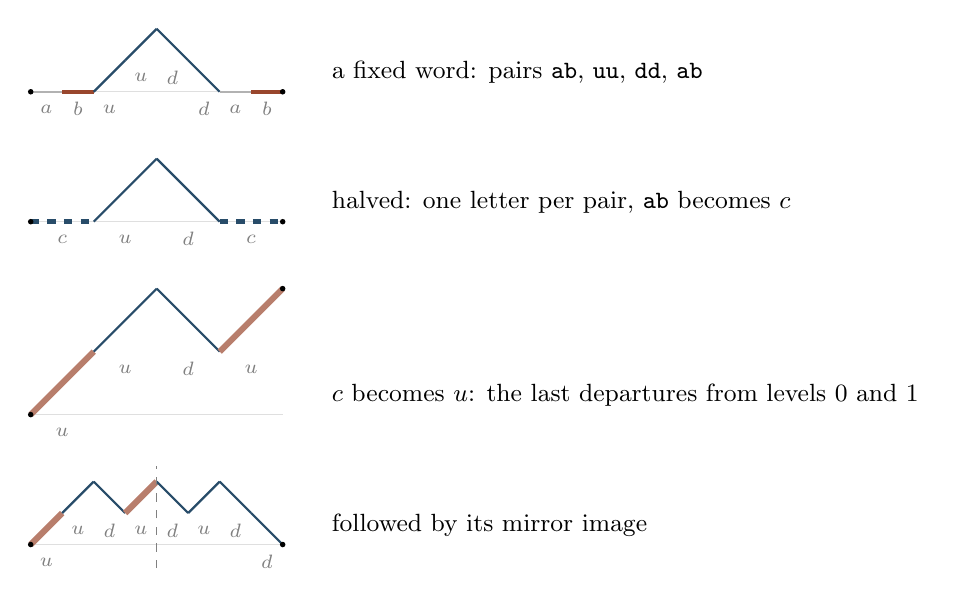
\begin{tikzpicture}[line join=round]
\draw[gray!25] (0,0.0) -- (3.2,0.0);
\draw[thick,gray!60] (0.000,0.000) -- (0.400,0.000);
\node[font=\scriptsize,gray] at (0.200,-0.220) {$a$};
\draw[ultra thick,rust] (0.400,0.000) -- (0.800,0.000);
\node[font=\scriptsize,gray] at (0.600,-0.220) {$b$};
\draw[thick,inkblue] (0.800,0.000) -- (1.200,0.400);
\node[font=\scriptsize,gray] at (1.000,-0.220) {$u$};
\draw[thick,inkblue] (1.200,0.400) -- (1.600,0.800);
\node[font=\scriptsize,gray] at (1.400,0.180) {$u$};
\draw[thick,inkblue] (1.600,0.800) -- (2.000,0.400);
\node[font=\scriptsize,gray] at (1.800,0.180) {$d$};
\draw[thick,inkblue] (2.000,0.400) -- (2.400,0.000);
\node[font=\scriptsize,gray] at (2.200,-0.220) {$d$};
\draw[thick,gray!60] (2.400,0.000) -- (2.800,0.000);
\node[font=\scriptsize,gray] at (2.600,-0.220) {$a$};
\draw[ultra thick,rust] (2.800,0.000) -- (3.200,0.000);
\node[font=\scriptsize,gray] at (3.000,-0.220) {$b$};
\fill (0.000,0.000) circle (1pt);
\fill (3.200,0.000) circle (1pt);
\node[font=\small,anchor=west] at (3.7,0.25) {a fixed word: pairs \texttt{ab}, \texttt{uu}, \texttt{dd}, \texttt{ab}};
\draw[gray!25] (0,-1.65) -- (3.2,-1.65);
\draw[ultra thick,inkblue,dashed] (0.000,-1.650) -- (0.800,-1.650);
\node[font=\scriptsize,gray] at (0.400,-1.870) {$c$};
\draw[thick,inkblue] (0.800,-1.650) -- (1.600,-0.850);
\node[font=\scriptsize,gray] at (1.200,-1.870) {$u$};
\draw[thick,inkblue] (1.600,-0.850) -- (2.400,-1.650);
\node[font=\scriptsize,gray] at (2.000,-1.870) {$d$};
\draw[ultra thick,inkblue,dashed] (2.400,-1.650) -- (3.200,-1.650);
\node[font=\scriptsize,gray] at (2.800,-1.870) {$c$};
\fill (0.000,-1.650) circle (1pt);
\fill (3.200,-1.650) circle (1pt);
\node[font=\small,anchor=west] at (3.7,-1.4) {halved: one letter per pair, \texttt{ab} becomes $c$};
\draw[gray!25] (0,-4.1) -- (3.2,-4.1);
\draw[thick,inkblue,line width=2.2pt,draw=rust!70] (0.000,-4.100) -- (0.800,-3.300);
\node[font=\scriptsize,gray] at (0.400,-4.320) {$u$};
\draw[thick,inkblue] (0.800,-3.300) -- (1.600,-2.500);
\node[font=\scriptsize,gray] at (1.200,-3.520) {$u$};
\draw[thick,inkblue] (1.600,-2.500) -- (2.400,-3.300);
\node[font=\scriptsize,gray] at (2.000,-3.520) {$d$};
\draw[thick,inkblue,line width=2.2pt,draw=rust!70] (2.400,-3.300) -- (3.200,-2.500);
\node[font=\scriptsize,gray] at (2.800,-3.520) {$u$};
\fill (0.000,-4.100) circle (1pt);
\fill (3.200,-2.500) circle (1pt);
\node[font=\small,anchor=west] at (3.7,-3.8499999999999996) {$c$ becomes $u$: the last departures from levels $0$ and $1$};
\draw[gray!25] (0,-5.75) -- (3.2,-5.75);
\draw[thick,inkblue,line width=2.2pt,draw=rust!70] (0.000,-5.750) -- (0.400,-5.350);
\node[font=\scriptsize,gray] at (0.200,-5.970) {$u$};
\draw[thick,inkblue] (0.400,-5.350) -- (0.800,-4.950);
\node[font=\scriptsize,gray] at (0.600,-5.570) {$u$};
\draw[thick,inkblue] (0.800,-4.950) -- (1.200,-5.350);
\node[font=\scriptsize,gray] at (1.000,-5.570) {$d$};
\draw[thick,inkblue,line width=2.2pt,draw=rust!70] (1.200,-5.350) -- (1.600,-4.950);
\node[font=\scriptsize,gray] at (1.400,-5.570) {$u$};
\draw[thick,inkblue] (1.600,-4.950) -- (2.000,-5.350);
\node[font=\scriptsize,gray] at (1.800,-5.570) {$d$};
\draw[thick,inkblue] (2.000,-5.350) -- (2.400,-4.950);
\node[font=\scriptsize,gray] at (2.200,-5.570) {$u$};
\draw[thick,inkblue] (2.400,-4.950) -- (2.800,-5.350);
\node[font=\scriptsize,gray] at (2.600,-5.570) {$d$};
\draw[thick,inkblue] (2.800,-5.350) -- (3.200,-5.750);
\node[font=\scriptsize,gray] at (3.000,-5.970) {$d$};
\fill (0.000,-5.750) circle (1pt);
\fill (3.200,-5.750) circle (1pt);
\node[font=\small,anchor=west] at (3.7,-5.5) {followed by its mirror image};
\draw[gray,dashed] (1.6,-6.05) -- (1.6,-4.75);
\end{tikzpicture}

\caption{Halving a fixed word, turning $c$ into $u$, and adding the mirror image. The two
highlighted steps are the last departures from levels $0$ and $1$; they are where the $c$ letters
were.}
\label{fig:halve}
\end{figure}

\begin{lemma}\label{lem:halve}
Halving, turning $c$ into $u$, keeping the lone last letter (if any) as a middle letter, and
appending the mirror image, is a bijection from the fixed words of length $n-1$ to the words of
Lemma~\ref{lem:word} that equal their mirror image. It keeps the number of letters from $\{u,b\}$.
\end{lemma}

\begin{proof}
Write $h$ for the word obtained after turning $c$ into $u$. Each $c$ occurs at height $0$ of the
halved word, and turning the $j$th one into $u$ raises everything after it by one more, so at that
step the new word climbs from $j-1$ to $j$ and afterwards stays at height at least $j$. The former
$c$ letters are therefore the last departures of $h$ from the levels $0,1,\dots,e-1$, where $e$ is
the final height of $h$. Conversely, in any word $h$ that never goes below its start and ends at
height $e$, marking the last departure from each level $0,\dots,e-1$ and turning those letters into
$c$ lowers the height after the $j$th mark by $j$. Before the $j$th mark the word sits at height
at least $j-1$, so the lowered word never goes below $0$, it is at height $0$ at every $c$, and it
ends at $0$. Doubling each letter back ($c\mapsto ab$) recovers the fixed word.

A word equal to its mirror image is $h$, then a middle letter when $n-1$ is odd (which the mirror
condition forces to be $a$ or $b$), then the mirror of $h$; it never goes below its start exactly
when $h$ does not. So the map is a bijection.

Count letters from $\{u,b\}$. In the fixed word there are $2\#uu+2\#bb+\#ab$ of them, plus one
for a final $b$. In the symmetric word, the mirror of $h$ has as many $u$ as $h$ has $d$, so there
are $\#u(h)+\#d(h)+2\#b(h)$, plus one for a middle $b$. Here $\#u(h)=\#uu+\#ab$, $\#d(h)=\#dd=\#uu$
and $\#b(h)=\#bb$, and the two counts agree.
\end{proof}

\begin{proof}[Proof of Theorem~\ref{thm:main}]
By~\eqref{eq:fixed}, $E_{n,k}-O_{n,k}$ is the number of fixed words with $k$ letters from $\{u,b\}$.
By Lemma~\ref{lem:halve} this is the number of mirror-symmetric words with $k$ such letters, and by
Lemma~\ref{lem:word} these are the words of the symmetric Dyck paths with $k$ valleys.
\end{proof}

In Figure~\ref{fig:three}, the fixed word $ab$ of \w{UUDDUD} halves to $c$, becomes $u$, and with
its mirror gives $ud$, the word of the symmetric path \w{UUDUDD}.

\section{Remarks}

The proof uses only the parity of the major index, together with the identity~\eqref{eq:FH} of
F\"urlinger and Hofbauer, which is quoted and not proved here. The cancellation is the same device,
swapping inside pairs of steps, that Martin Rubey used to evaluate weighted Motzkin paths in a
proof reported by Cigler~\cite[proof of the Lemma in Section 5]{Cig26b}; the new ingredients are the
valley coordinates, which make the sign of a Dyck path local, and the last-departure bijection.

The involution and the bijection do not commute with taking mirror images, and Section~2
shows that no cancellation can fix exactly the symmetric paths. A single map from the even paths
to the odd paths together with the symmetric ones, which Taylor's reformulation also invites, is
not constructed here.

\paragraph{Verification.} The whole argument, from Dyck paths written as lists of steps to
Theorem~\ref{thm:main}, is formalised in Lean~4 with Mathlib~\cite{mathlib}, using only the standard
axioms; identity~\eqref{eq:FH} is the one statement taken from the literature. A Python program
checks every claim of Sections~3 to~5 for all paths with $n\le 12$. An independent program, sharing
no code with it, recomputes the examples in the text, confirms Theorem~\ref{thm:main} and its
agreement with the right side of~\eqref{eq:FH} at $q=-1$ for $n\le 10$, and checks~\eqref{eq:FH}
itself coefficient by coefficient for $n\le 8$. Both, with the Lean files, are at
\url{https://github.com/jvvk/mathematics/tree/main/even-and-odd-dyck-paths}.

\paragraph{Acknowledgements.} Johann Cigler posed the question; Peter Taylor, Darij Grinberg,
Sam Hopkins, Martin Rubey and Fedor Petrov contributed to the discussion on MathOverflow.
Anthropic's Claude (Opus~5.5) was used to find the proof, write the Lean formalisation and the
checking programs, and draft this text. The author takes responsibility for the content.

\begin{thebibliography}{9}
\bibitem{Cig26} J.~Cigler, Symmetric Dyck paths and $q$-Narayana numbers, arXiv:2601.08366 (2026).
\bibitem{Cig26b} J.~Cigler, Continued fractions related to Narayana polynomials, arXiv:2604.24207 (2026).
\bibitem{MO} J.~Cigler, Combinatorial interpretation of $q$-Narayana numbers for $q=-1$,
MathOverflow question 501839 (20 October 2025), \url{https://mathoverflow.net/q/501839},
accessed 10 October 2026.
\bibitem{FH} J.~F\"urlinger and J.~Hofbauer, $q$-Catalan numbers, \emph{J. Combin. Theory Ser. A}
\textbf{40} (1985) 248--264, \href{https://doi.org/10.1016/0097-3165(85)90089-5}{doi:10.1016/0097-3165(85)90089-5}.
\bibitem{RSW} V.~Reiner, D.~Stanton and D.~White, The cyclic sieving phenomenon, \emph{J. Combin.
Theory Ser. A} \textbf{108} (2004) 17--50, \href{https://doi.org/10.1016/j.jcta.2004.04.009}{doi:10.1016/j.jcta.2004.04.009}.
\bibitem{Stem} J.~R.~Stembridge, Some hidden relations involving the ten symmetry classes of plane
partitions, \emph{J. Combin. Theory Ser. A} \textbf{68} (1994) 372--409,
\href{https://doi.org/10.1016/0097-3165(94)90112-0}{doi:10.1016/0097-3165(94)90112-0}.
\bibitem{mathlib} The mathlib Community, The Lean mathematical library, in \emph{Proceedings of the
9th ACM SIGPLAN International Conference on Certified Programs and Proofs (CPP 2020)}, 367--381,
\href{https://doi.org/10.1145/3372885.3373824}{doi:10.1145/3372885.3373824}.
\end{thebibliography}

\bigskip
\noindent Vamshi Jandhyala, London, UK.

\end{document}
